\section{Descrição do Problema}

\paragraph O problema da Gold Star consiste num puzzle que exibe um conjunto de equações em forma de estrela cujo objetivo é preencher os círculos vazios das equações de modo a que estas se tornam verdadeiras quando lidas da esquerda para a direita. A resolução do problema é preencher com operadores aritméticos (+, - , *, /) e dígitos de 0 a 9 os círculos vazios da estrela, sendo que cada dígito é utilizado uma única vez. Sendo o caso base uma estrela de 5 pontos, existem 5 equações que partilham as 10 varáveis numéricas e os 10 operadores aritméticos, obtendo uma estrela como a que se apresenta na Figura \ref{fig:configuracao_estrela_5_pontas} .

\begin{figure}[!htb]
\hfill
\subfigure[não resolvida]{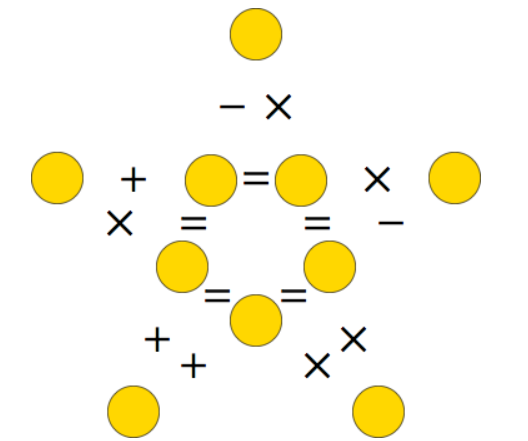
\includegraphics[width=6.4cm]{images/estrela_inicial.png}}\label{fig1}
\hfill
\subfigure[resolvida]{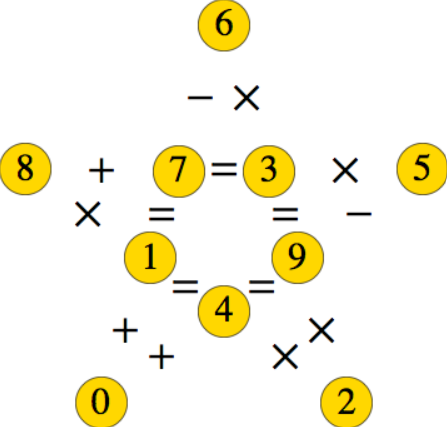
\includegraphics[width=5cm]{images/star_solved.png}}
\hfill
\caption{Exemplo da configuração da estrela de 5 pontas}\label{fig:configuracao_estrela_5_pontas}
\end{figure}


